\chapter{Development}
\label{chapter:desenvolvimento}

This chapter describes the architecture and implementation of \textit{G-FShield}. The contribution presented here is architectural and software-engineering-oriented: it integrates initial-solution construction, local-search refinement, messaging, persistence, and operational inspection. The feature-selection and search algorithms derive from previous work and are not claimed as new.

\section{Overview and Input Contract}

\textit{G-FShield} was structured into three layers: a web operations layer, an orchestration and persistence layer, and a distributed execution layer. The first presents observed state and receives commands; the second centralizes the \ac{api}, database, \textit{cache}, and messaging integration; and the third executes the distributed restricted candidate list generation (\ac{drg}) and distributed local search (\ac{dls}). Figure~\ref{fig:arquitetura-resumo} summarizes these boundaries.

\begin{landscape}
\begin{figure}[p]
  \centering
  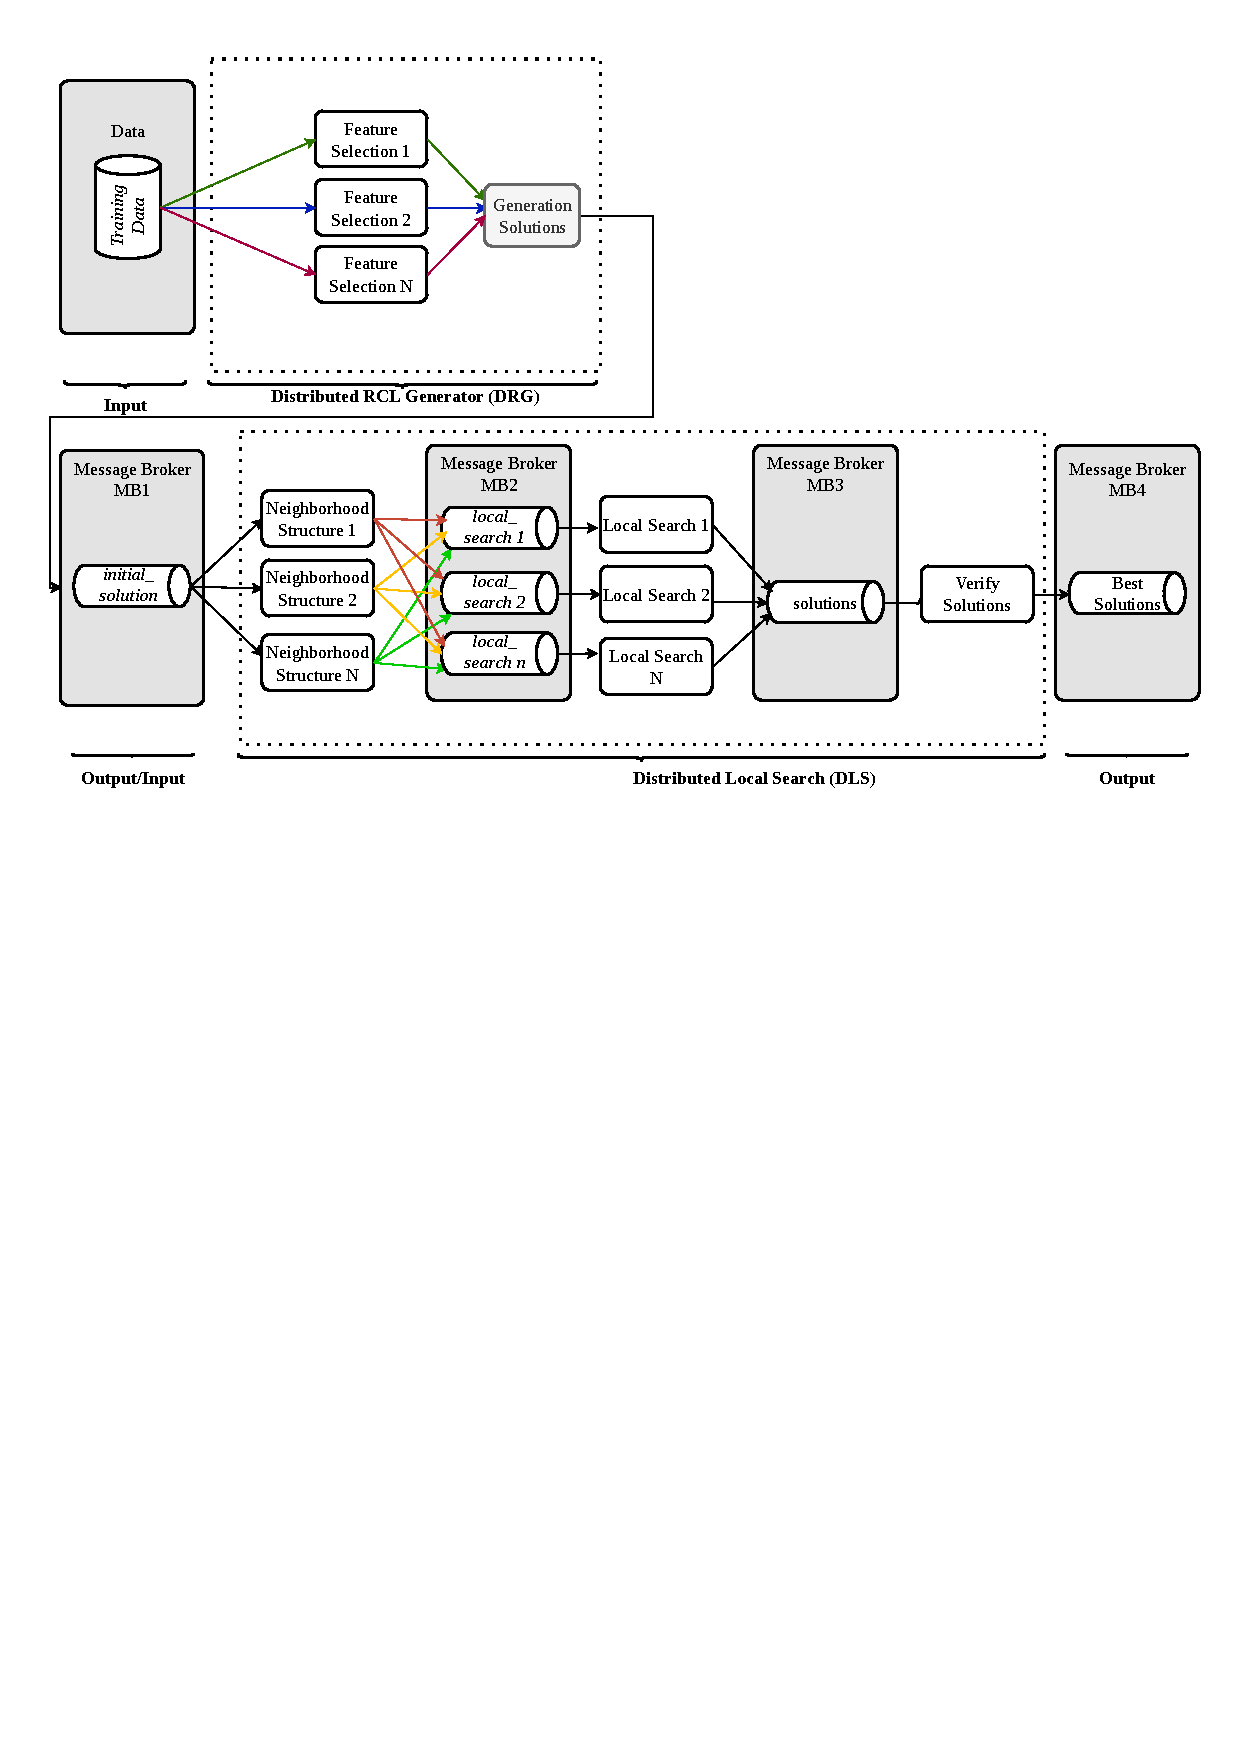
\includegraphics[trim=0 420bp 0 0,clip,width=.96\linewidth,height=.82\textheight,keepaspectratio]{fig/gfshield/arquitetura-full-summary.pdf}
  \caption{Summary of the \textit{G-FShield} architecture; the blank margin in the original file is removed only by the LaTeX inclusion.}
  \label{fig:arquitetura-resumo}
\end{figure}
\end{landscape}

Independence from the data source is conditional on a concrete contract. The algorithmic API receives two distinct ARFF files, one for training and one for scoring candidates, accessible at \texttt{/datasets}. They must share the same schema and keep the label as the last attribute. In the formal campaign, the second file is validation data; the held-out test is accessed only by the final evaluator. The Weka reader assigns the last attribute as the class, and predictors use one-based identifiers. The application accepts J48, Naive Bayes, and Random Forest; the campaign fixes J48.

Consequently, network traffic, protocols, or logs are not consumed in raw form: they must first be transformed into labeled matrices that satisfy this contract. Generality is therefore an architectural and input-format property, not empirical evidence of performance across heterogeneous sources. Historical CSV files reference \texttt{erenoall.arff}, whereas the current script uses the ERENO~1k split; without a manifest, one configuration cannot be attributed to the other. Moreover, in the available \texttt{erenoall.arff}, \textit{grayhole} occupies index zero and \textit{normal} index one, conflicting with the code's \texttt{normalClass} name. This mapping must be corrected by label before a new evaluation.

Each request supplies the training and testing files, classifier, number of generations, RCL cutoff, initial sample size, VND or RVND strategy, enabled local searches, and optional iteration limits. These fields form the configuration unit propagated between services. Each solution also receives a random \texttt{seedId}, which correlates the refinements derived from it.

\section{Architectural Drivers and Decisions}

The decomposition was guided by six drivers: throughput, decoupling, traceability, persistence, inspection of intermediate results, and the possibility of operational evolution. Table~\ref{tab:architecture-drivers} makes the relationship between these drivers and the adopted decisions explicit. Service decomposition and asynchronous communication follow established principles of distributed systems and microservice architectures~\cite{Tanenbaum2007Distributed,Newman2021,Kreps2011}.

\begin{table}[!htb]
  \centering
  \small
  \caption{Architectural drivers, decisions, and limits.}
  \label{tab:architecture-drivers}
  \begin{tabularx}{\linewidth}{@{}p{.18\linewidth}X X@{}}
    \toprule
    \textbf{Driver} & \textbf{Design decision} & \textbf{Scope of evidence} \\
    \midrule
    Throughput & Execute the four rankings in independent services and forward seeds to decoupled search operators. & The evaluation measures the deployed configuration; it does not demonstrate efficiency under equal resources. \\
    Decoupling & Use Kafka topics between construction, controllers, operators, verifier, and monitor. & Temporal coupling is reduced, but robustness under failure was not experimentally measured. \\
    Traceability & Propagate \texttt{seedId}, algorithm, search, iterations, feature sets, and metrics. & The sequence observed by the monitor can be reconstructed; flow completeness is not proven. \\
    Persistence & Store launches, runs, events, and aggregates in PostgreSQL and CSVs in the metrics volume. & Redis is a \textit{cache}; it does not replace persistent storage. \\
    Intermediate inspection & Publish selected progress, refined solutions, and observed best solutions. & The interface presents telemetry; it does not make the algorithm explainable. \\
    Operational evolution & Isolate responsibilities to allow service-level replication and replacement. & Scalability and fault tolerance are design objectives, not demonstrated results. \\
    \bottomrule
  \end{tabularx}
\end{table}

The construction and refinement phases differ in cost and resource-use patterns. They were therefore separated into services with their own CPU, memory, and concurrency limits. This separation permits one responsibility to be observed and changed without incorporating the entire search into a single process. It also makes it possible to increase the number of instances of a service; however, the relationship between replicas, throughput, and cost requires a dedicated scaling experiment.

Persistence and event history were adopted to reduce reliance on state kept only in memory. The evaluated configuration, however, uses one Kafka broker and replication factor one. High availability or fault tolerance therefore cannot be inferred from the decomposition. Those properties would require fault injection and verification of redelivery, idempotency, recovery, and reprocessing.

\section{Distributed Restricted Candidate List Generation}

In the \ac{drg} stage, four independent services calculate \ac{ig}, \ac{gr}, \ac{su}, and ReliefF. Each service scores only training predictors, sorts them in descending order, and forms its own RCL from the first \texttt{rclCutoff} elements; the class attribute in the last position is excluded from ranking. There is no aggregator that merges the four rankings into one list. A request containing several metrics launches independent branches that publish initial solutions to the same topic.

Construction follows the principle of an RCL combined with random choice, which is characteristic of GRASP~\cite{ResendeRibeiro2010}. The adaptation to feature selection and the DRG stages used here derive from GRASP-FS and its distributed extensions~\cite{quincozes2020grasp,quincozes2021performance,quincozes2022extended,Naves2023DRG}. These references support the algorithmic decision; microservice references support only the implementation decomposition.

\begin{landscape}
\begin{figure}[p]
  \centering
  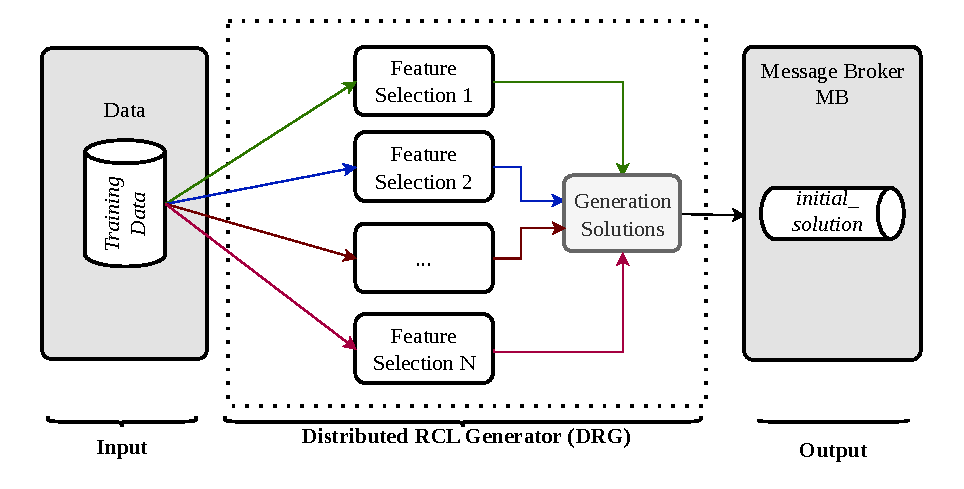
\includegraphics[width=.96\linewidth,height=.82\textheight,keepaspectratio]{fig/gfshield/generic-drg.pdf}
  \caption{Generic architecture of the \ac{drg} stage.}
  \label{fig:drg-generic}
\end{figure}
\end{landscape}

\begin{landscape}
\begin{figure}[p]
  \centering
  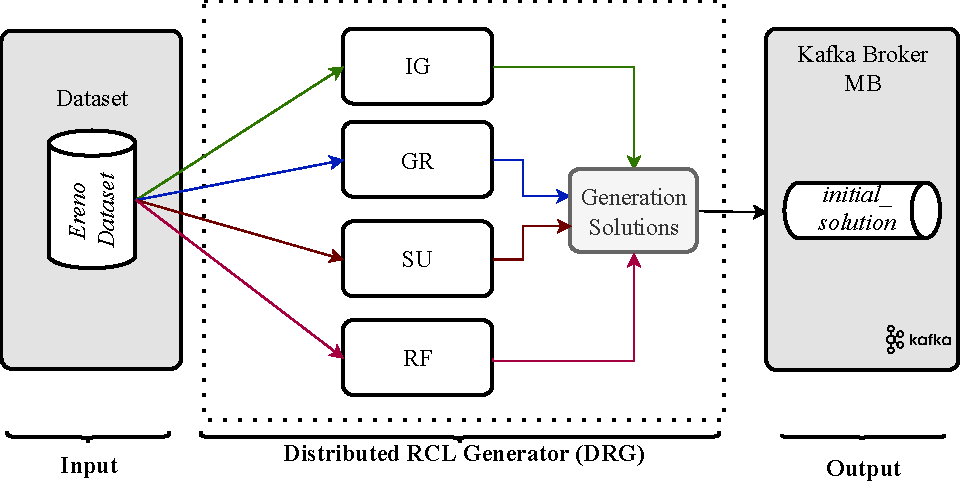
\includegraphics[width=.96\linewidth,height=.82\textheight,keepaspectratio]{fig/gfshield/drg-specific.pdf}
  \caption{Concrete \ac{drg} instantiation with the four implemented metrics.}
  \label{fig:drg-specific}
\end{figure}
\end{landscape}

For each generation, the service copies its RCL and samples \texttt{sampleSize} positions uniformly without replacement from that copy. In the formal campaign, the generator is initialized by \texttt{CAMPAIGN\_RANDOM\_SEED}; \texttt{seedId} identifies the solution, while \texttt{campaignId}, \texttt{runId}, \texttt{requestId}, and the numeric seed preserve provenance. The subset is evaluated on reduced training and validation data; the held-out test set does not participate in search. The published message preserves the subset, RCL, internal metrics, and refinement configuration.

Listing~\ref{lst:drg-pseudocode} presents this behavior as pseudocode. \texttt{metric} identifies one of the four branches. Parameters map as follows:
\begin{itemize}
  \item \texttt{G}: \texttt{maxGenerations};
  \item \texttt{k}: \texttt{rclCutoff};
  \item \texttt{s}: \texttt{sampleSize}.
\end{itemize}

\begin{lstlisting}[caption={Implemented RCL formation and randomized construction in the DRG.},label={lst:drg-pseudocode},basicstyle=\ttfamily\small,breaklines=true,columns=fullflexible]
procedure DRG(trainFile, validationFile, metric, G, k, s, classifier,
              neighborhood, enabledSearches, iterationLimits, runSeed)
  train <- readARFF(trainFile); train.class <- lastAttribute
  valid <- readARFF(validationFile); valid.class <- lastAttribute
  rng <- PseudoRandomGenerator(runSeed)

  scored <- empty list
  for each predictor a in train, excluding the class do
    scored.append((metric(train, a), oneBasedIndex(a)))
  end for
  ranking <- sortDescending(scored)
  rcl <- first min(k, size(ranking)) feature identifiers

  for generation <- 1 to G do
    pool <- copy(rcl)
    selected <- empty list
    repeat min(s, size(pool)) times
      p <- UniformInteger(rng, 1, size(pool))
      selected.append(removeAt(pool, p))
    end repeat

    seedId <- randomUUID()
    scores <- trainAndValidate(classifier, train, valid, selected)
    appendServiceMetricsCSV(selected, scores, classifier,
                            trainFile, validationFile)
    publish(INITIAL_SOLUTION_TOPIC,
            {seedId, selected, rcl, scores, metric,
             neighborhood, enabledSearches, iterationLimits})
  end for
end procedure
\end{lstlisting}

\section{Distributed Local Search}

The \ac{vnd} and \ac{rvnd} controllers receive each initial solution and forward messages to the Bit Flip, \ac{iwss}, and \ac{iwssr} operators. VND visits the enabled searches in configured order, compares the best cycle result with its baseline, and restarts the cycle when an improvement occurs and dispatch budget remains. RVND randomly selects an enabled search at each step and continues until the iteration limit. VND and its randomized variant are grounded in the variable-neighborhood and RVND literature~\cite{MladenovicHansen1997VNS,DuarteEtAl2018VND,SUBRAMANIAN20101899}; distribution of these operators follows GDLS-FS~\cite{Silva2023GDLSFS}.

Bit Flip randomly exchanges one subset attribute with one attribute in the candidate list at each iteration. IWSS sequentially adds the first still-available attribute and preserves the best evaluated subset. IWSSR performs the addition move and, for every position of the resulting subset, evaluates the corresponding removal, retaining the best replacement. These neighborhood operators follow the GRASP-FS assessments~\cite{quincozes2020grasp,quincozes2021performance,quincozes2022extended}. The RCL forwarded to DLS still contains initial-solution attributes, but the campaign canonicalizes the final solution and rejects empty, invalid, or duplicated subsets. Operators train on training data, score candidates on validation data, and publish results to \texttt{SOLUTIONS\_TOPIC}. The verifier keeps the greatest internal F1 per \texttt{seedId} and publishes strict improvements to \texttt{BEST\_SOLUTION\_TOPIC}; this is the best observed result, not a global certificate of optimality.

\begin{landscape}
\begin{figure}[p]
  \centering
  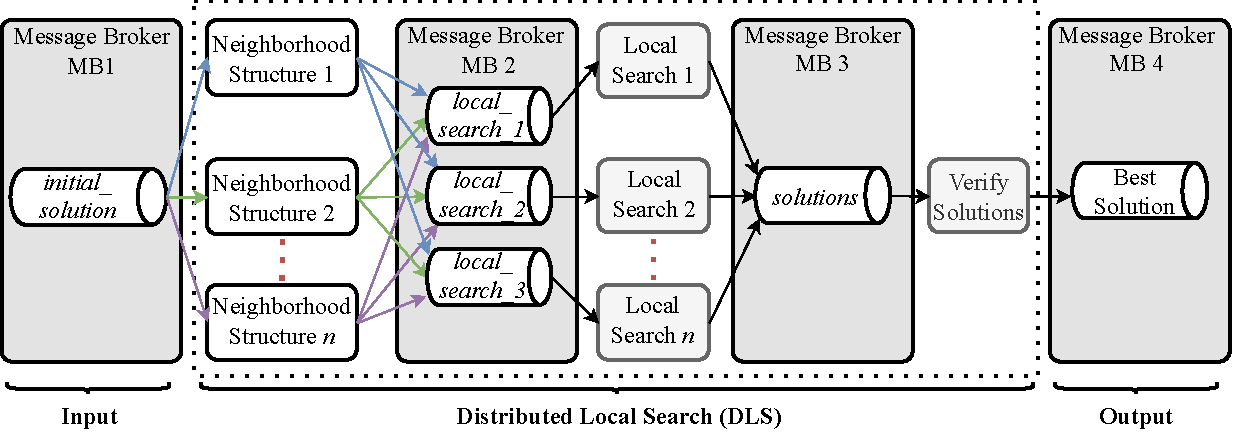
\includegraphics[width=.96\linewidth,height=.82\textheight,keepaspectratio]{fig/gfshield/dls-generic.pdf}
  \caption{Generic architecture of the \ac{dls} stage.}
  \label{fig:dls-generic}
\end{figure}
\end{landscape}

\begin{landscape}
\begin{figure}[p]
  \centering
  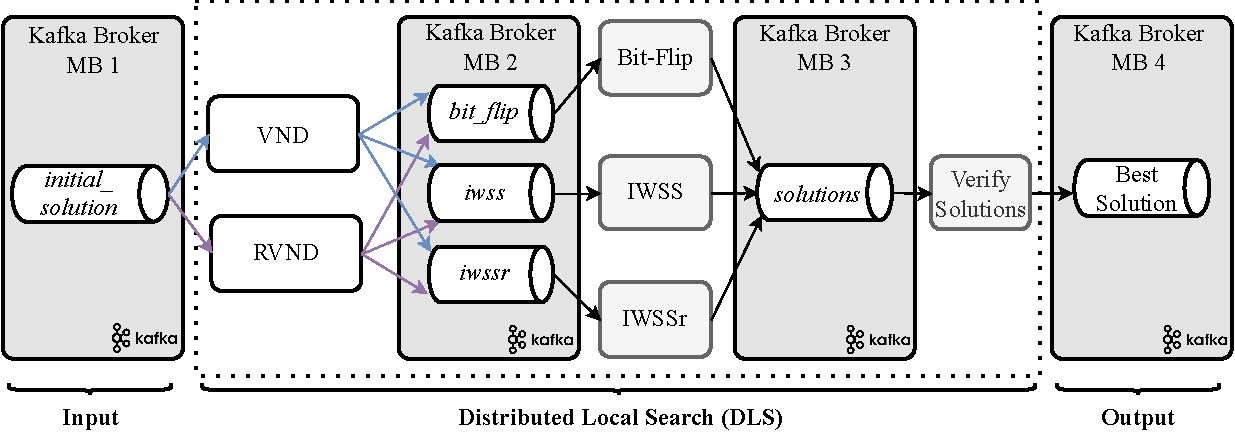
\includegraphics[width=.96\linewidth,height=.82\textheight,keepaspectratio]{fig/gfshield/dls-specific.pdf}
  \caption{Concrete \ac{dls} instantiation with the implemented controllers and operators.}
  \label{fig:dls-specific}
\end{figure}
\end{landscape}

Listing~\ref{lst:dls-pseudocode} summarizes the effective orchestration. The VND budget is the configured number of cycles multiplied by the number of enabled searches; RVND uses the iteration limit directly. Both controllers default to ten when the request does not provide a limit.

\begin{lstlisting}[caption={Implemented distributed refinement and verification in the DLS.},label={lst:dls-pseudocode},basicstyle=\ttfamily\small,breaklines=true,columns=fullflexible]
on INITIAL_SOLUTION_TOPIC or NEIGHBORHOOD_RESTART_TOPIC receive seed
  best <- seed
  searches <- configured searches or [BIT_FLIP, IWSS, IWSSR]

  if seed.neighborhood = VND then
    dispatchBudget <- maxCycles * size(searches)
    repeat while dispatchBudget remains
      baseline <- best.F1
      for each search in searches in configured order do
        candidate <- dispatchAndReceive(search, best)
        best <- argmaxF1(best, candidate)
        dispatches <- dispatches + 1
      end for
      if best.F1 <= baseline then stop
    end repeat
  else if seed.neighborhood = RVND then
    repeat until maxIterations dispatches
      search <- UniformChoice(searches)
      candidate <- dispatchAndReceive(search, best)
      best <- argmaxF1(best, candidate)
      dispatches <- dispatches + 1
    end repeat
  end if

  for each candidate received by verifier do
    if bestSeen[candidate.seedId] is undefined or
       candidate.F1 > bestSeen[candidate.seedId].F1 then
      bestSeen[candidate.seedId] <- candidate
      publish(BEST_SOLUTION_TOPIC, candidate)
    end if
  end for
end receive
\end{lstlisting}

The formal protocol initializes construction, Bit Flip, and RVND with the run's numeric seed and persists it separately from UUID \texttt{seedId}. This makes the pseudorandom sequence repeatable in the versioned environment; concurrency, message ordering, and platform may still introduce variation, so every result also preserves timestamps, command, and artifacts.

\section{Event-Driven Orchestration}

Kafka decouples producers and consumers through the following topic groups:
\begin{itemize}
  \item construction: \path{INITIAL_SOLUTION_TOPIC};
  \item operators: \path{BIT_FLIP_TOPIC}, \path{IWSS_TOPIC}, and \path{IWSSR_TOPIC};
  \item coordination: \path{SOLUTIONS_TOPIC} and \path{NEIGHBORHOOD_RESTART_TOPIC};
  \item monitored progress: \path{LOCAL_SEARCH_PROGRESS_TOPIC};
  \item best observed result: \path{BEST_SOLUTION_TOPIC}.
\end{itemize}
The key of a solution message is the \texttt{seedId}, when available, and observed events feed the monitor~\cite{Kreps2011}.

\begin{landscape}
\begin{figure}[p]
  \centering
  \includegraphics[width=.96\linewidth,height=.82\textheight,keepaspectratio]{fig/gfshield/gfshield-deployment-topology.pdf}
  \caption{Deployment topology and execution boundaries of \textit{G-FShield}.}
  \label{fig:deployment-topology}
\end{figure}
\end{landscape}

Kafka is configured as an execution event log, but potential durability is not equivalent to demonstrated recovery. The configuration enables automatic topic creation, six partitions, and replication factor one. Message loss or duplication, event completeness, instrumentation cost, post-restart behavior, consumer recovery, and reprocessing were not measured. Resilience and fault tolerance therefore remain design objectives.

\section{Persisted Telemetry and Web Layer}

Observability in this work means the ability to inspect recorded external execution state. It does not mean causally explaining classifier decisions. The \ac{api} monitor consumes five topics of interest: initial solution, neighborhood restart, local-search progress, refined solution, and best solution. Each persisted event contains a type, JSON payload, and backend ingestion timestamp, as well as topic, stage, status, \texttt{seedId}, \texttt{requestId}, partition, and offset when available. A fingerprint prevents reinserting the same observed event. In the formal campaign, \texttt{campaignId}, \texttt{runId}, \texttt{requestId}, \texttt{seedId}, producer UTC timestamp, and monotonic elapsed time are propagated in experimental objects.

PostgreSQL maintains three principal levels: the requested launch, current run per \texttt{seedId}, and associated event history. Run state includes RCL algorithm, classifier, local search, neighborhood, files, iterations, F1, accuracy, precision, recall, CPU, memory, time, and feature sets. Materialized read models aggregate topics, algorithms, resources, and timeline intervals. Redis temporarily stores frequently requested responses; PostgreSQL is the persistent source.

The Java services also write per-component CSVs to the \texttt{/metrics} volume. These files contain the subset, F1, accuracy, precision, recall, time, CPU, memory, classifier, and filenames. Because the current CSVs do not record \texttt{seedId}, direct correlation with the web history must not be assumed. Java and Node logs are emitted to \textit{stdout}; Compose configures no log store, retention policy, or collector such as Loki/ELK. Events and metrics are therefore persisted by the application, but log persistence depends on the external runtime and was not demonstrated.

The combination of identifiers, events, and timestamps reconstructs the timeline that reached the monitor and permits states of the same seed to be compared. It does not guarantee that every produced event was captured. In the formal campaign, the numeric seed, \texttt{runId}, and checksums complement this telemetry; monitor completeness and reproduction on different hardware remain limited.

\begin{figure}[p]
  \centering
  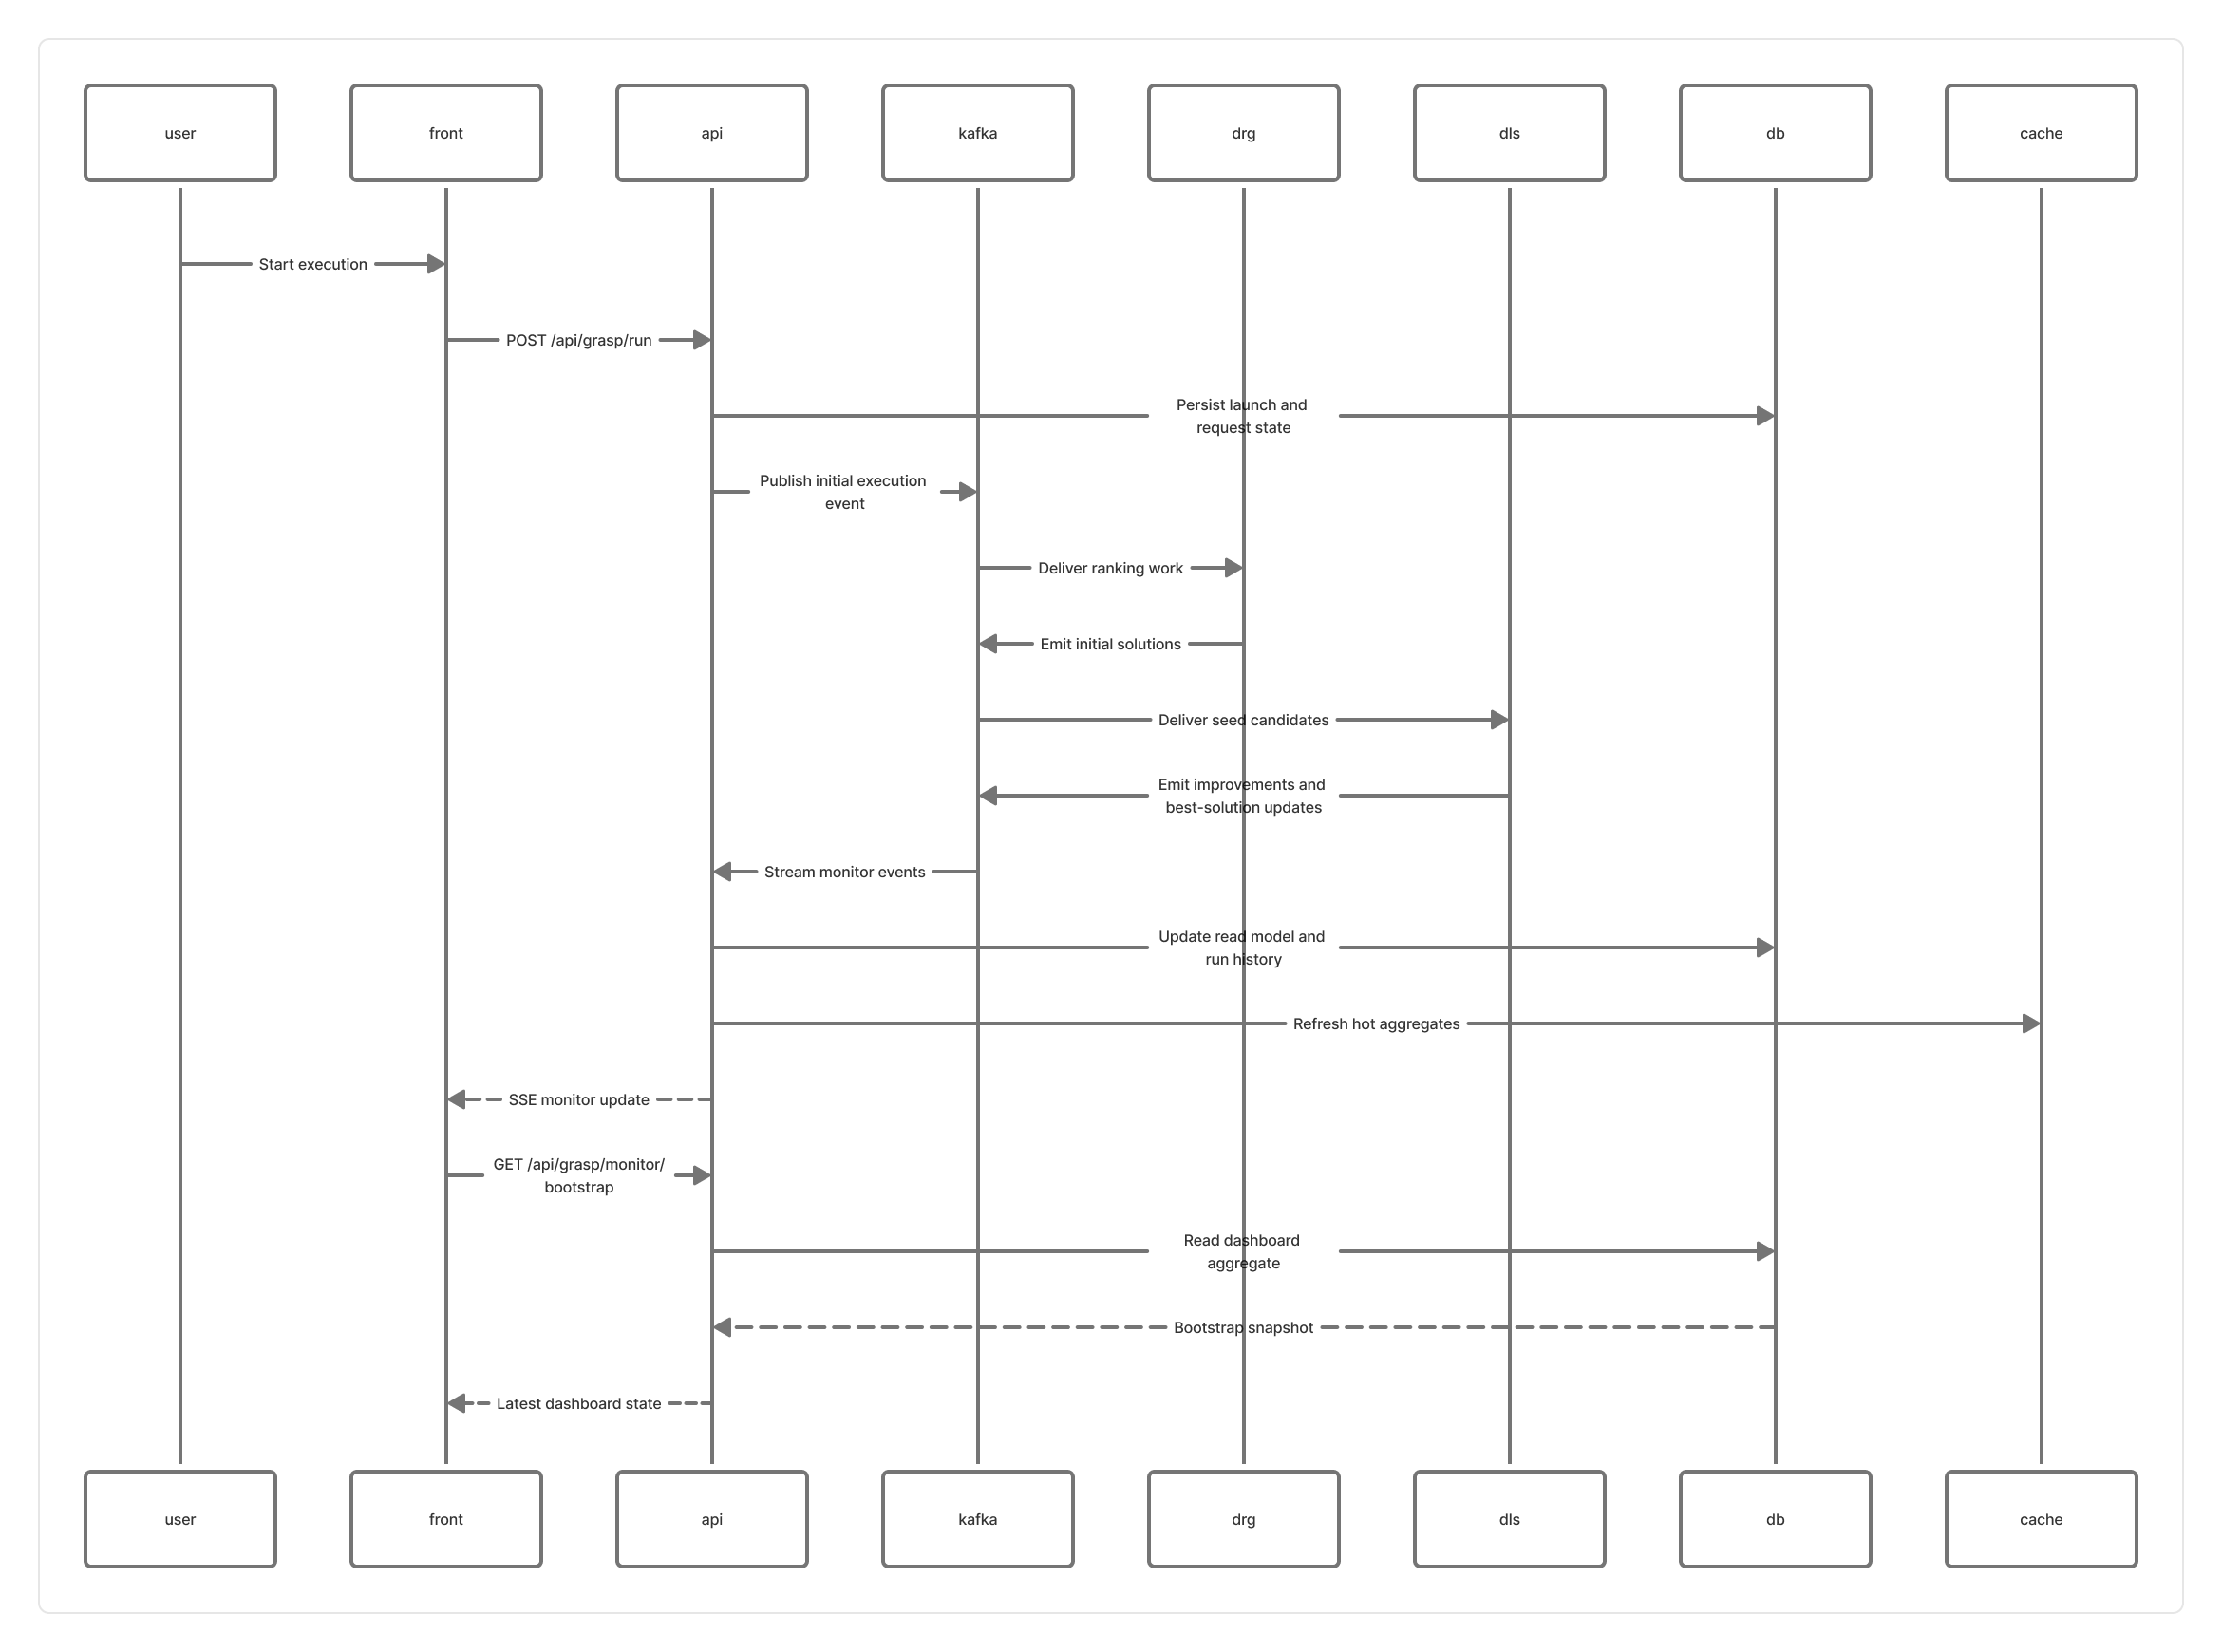
\includegraphics[width=\linewidth,height=.74\textheight,keepaspectratio]{fig/gfshield/g-fshield-execution-lifecycle.png}
  \caption{Execution lifecycle of \textit{G-FShield}, from the request to the states shown in the interface.}
  \label{fig:execution-lifecycle}
\end{figure}

\begin{figure}[p]
  \centering
  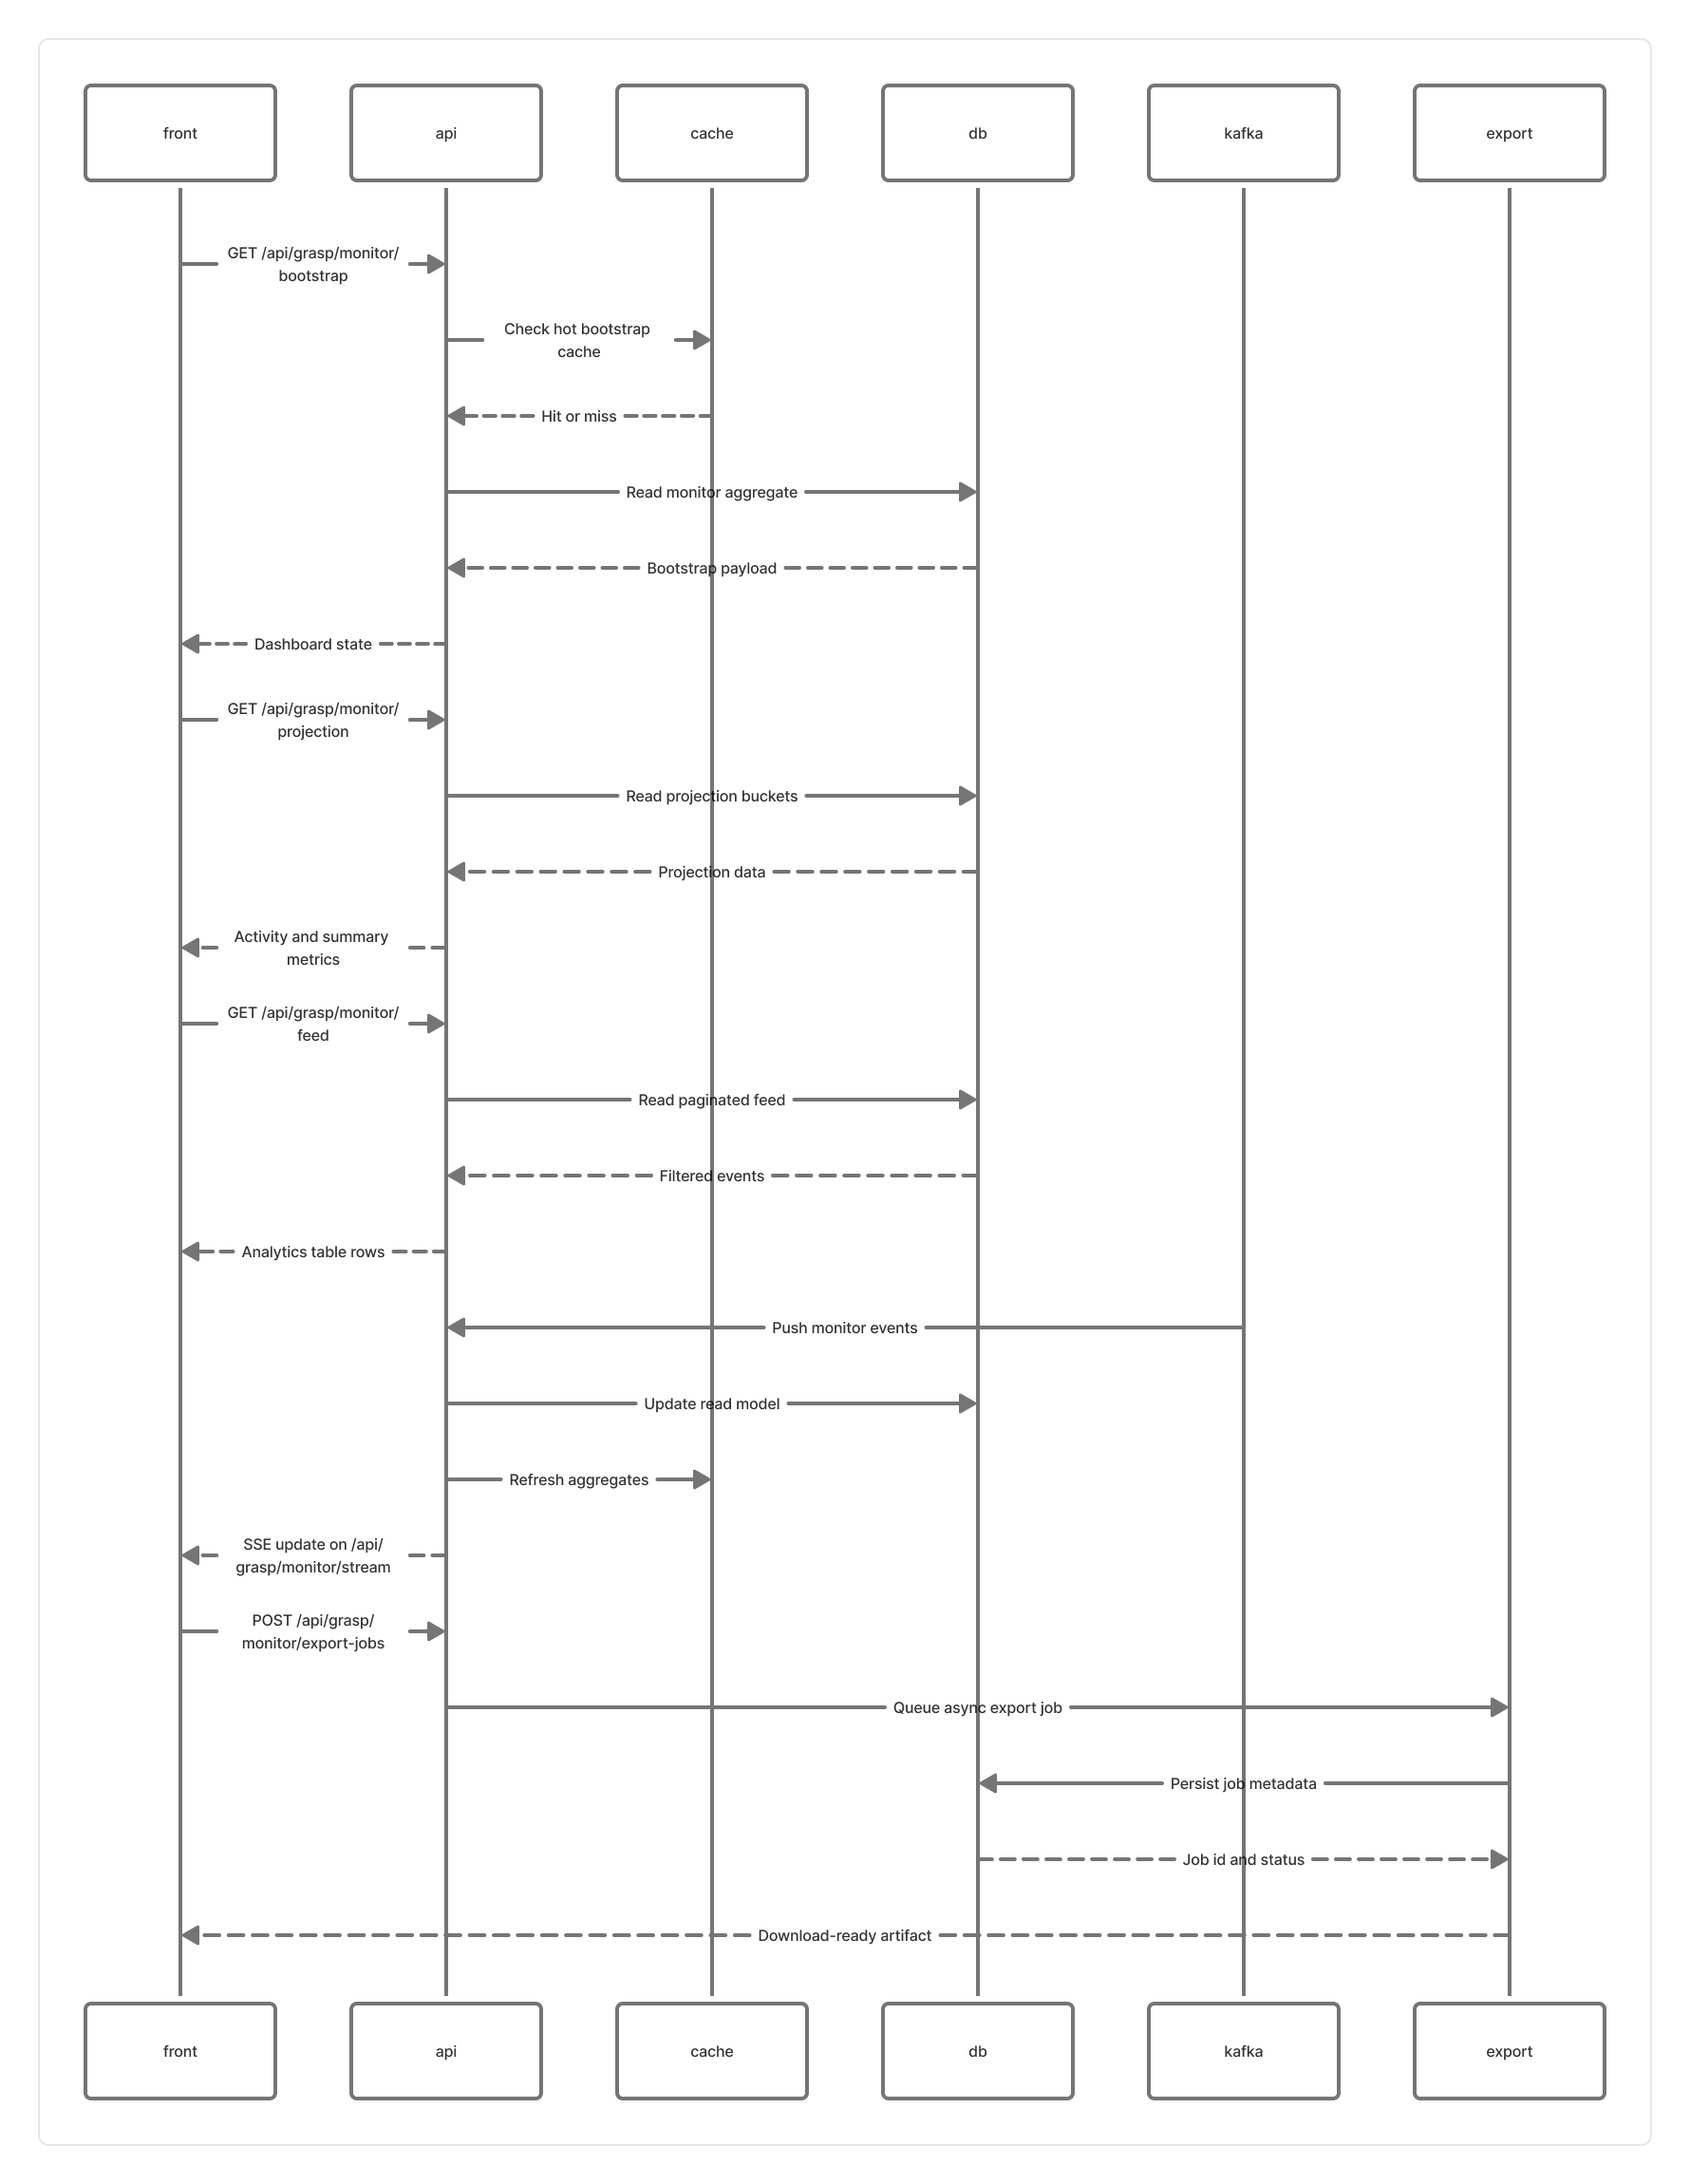
\includegraphics[width=\linewidth,height=.82\textheight,keepaspectratio]{fig/gfshield/g-fshield-monitoring-pipeline.png}
  \caption{Ingestion, persistence, and presentation pipeline for observed telemetry.}
  \label{fig:monitoring-pipeline}
\end{figure}

The web implementation uses React and Vite in the client; Express and Swagger in the \ac{api}; PostgreSQL for persistence; and Redis as an optional \textit{cache}. The interface queries summaries, paginated events, timelines, and CSV or JSON exports. These technologies describe the implementation; by themselves, they do not prove productivity, stability, responsiveness, or performance.

\begin{figure}[p]
  \centering
  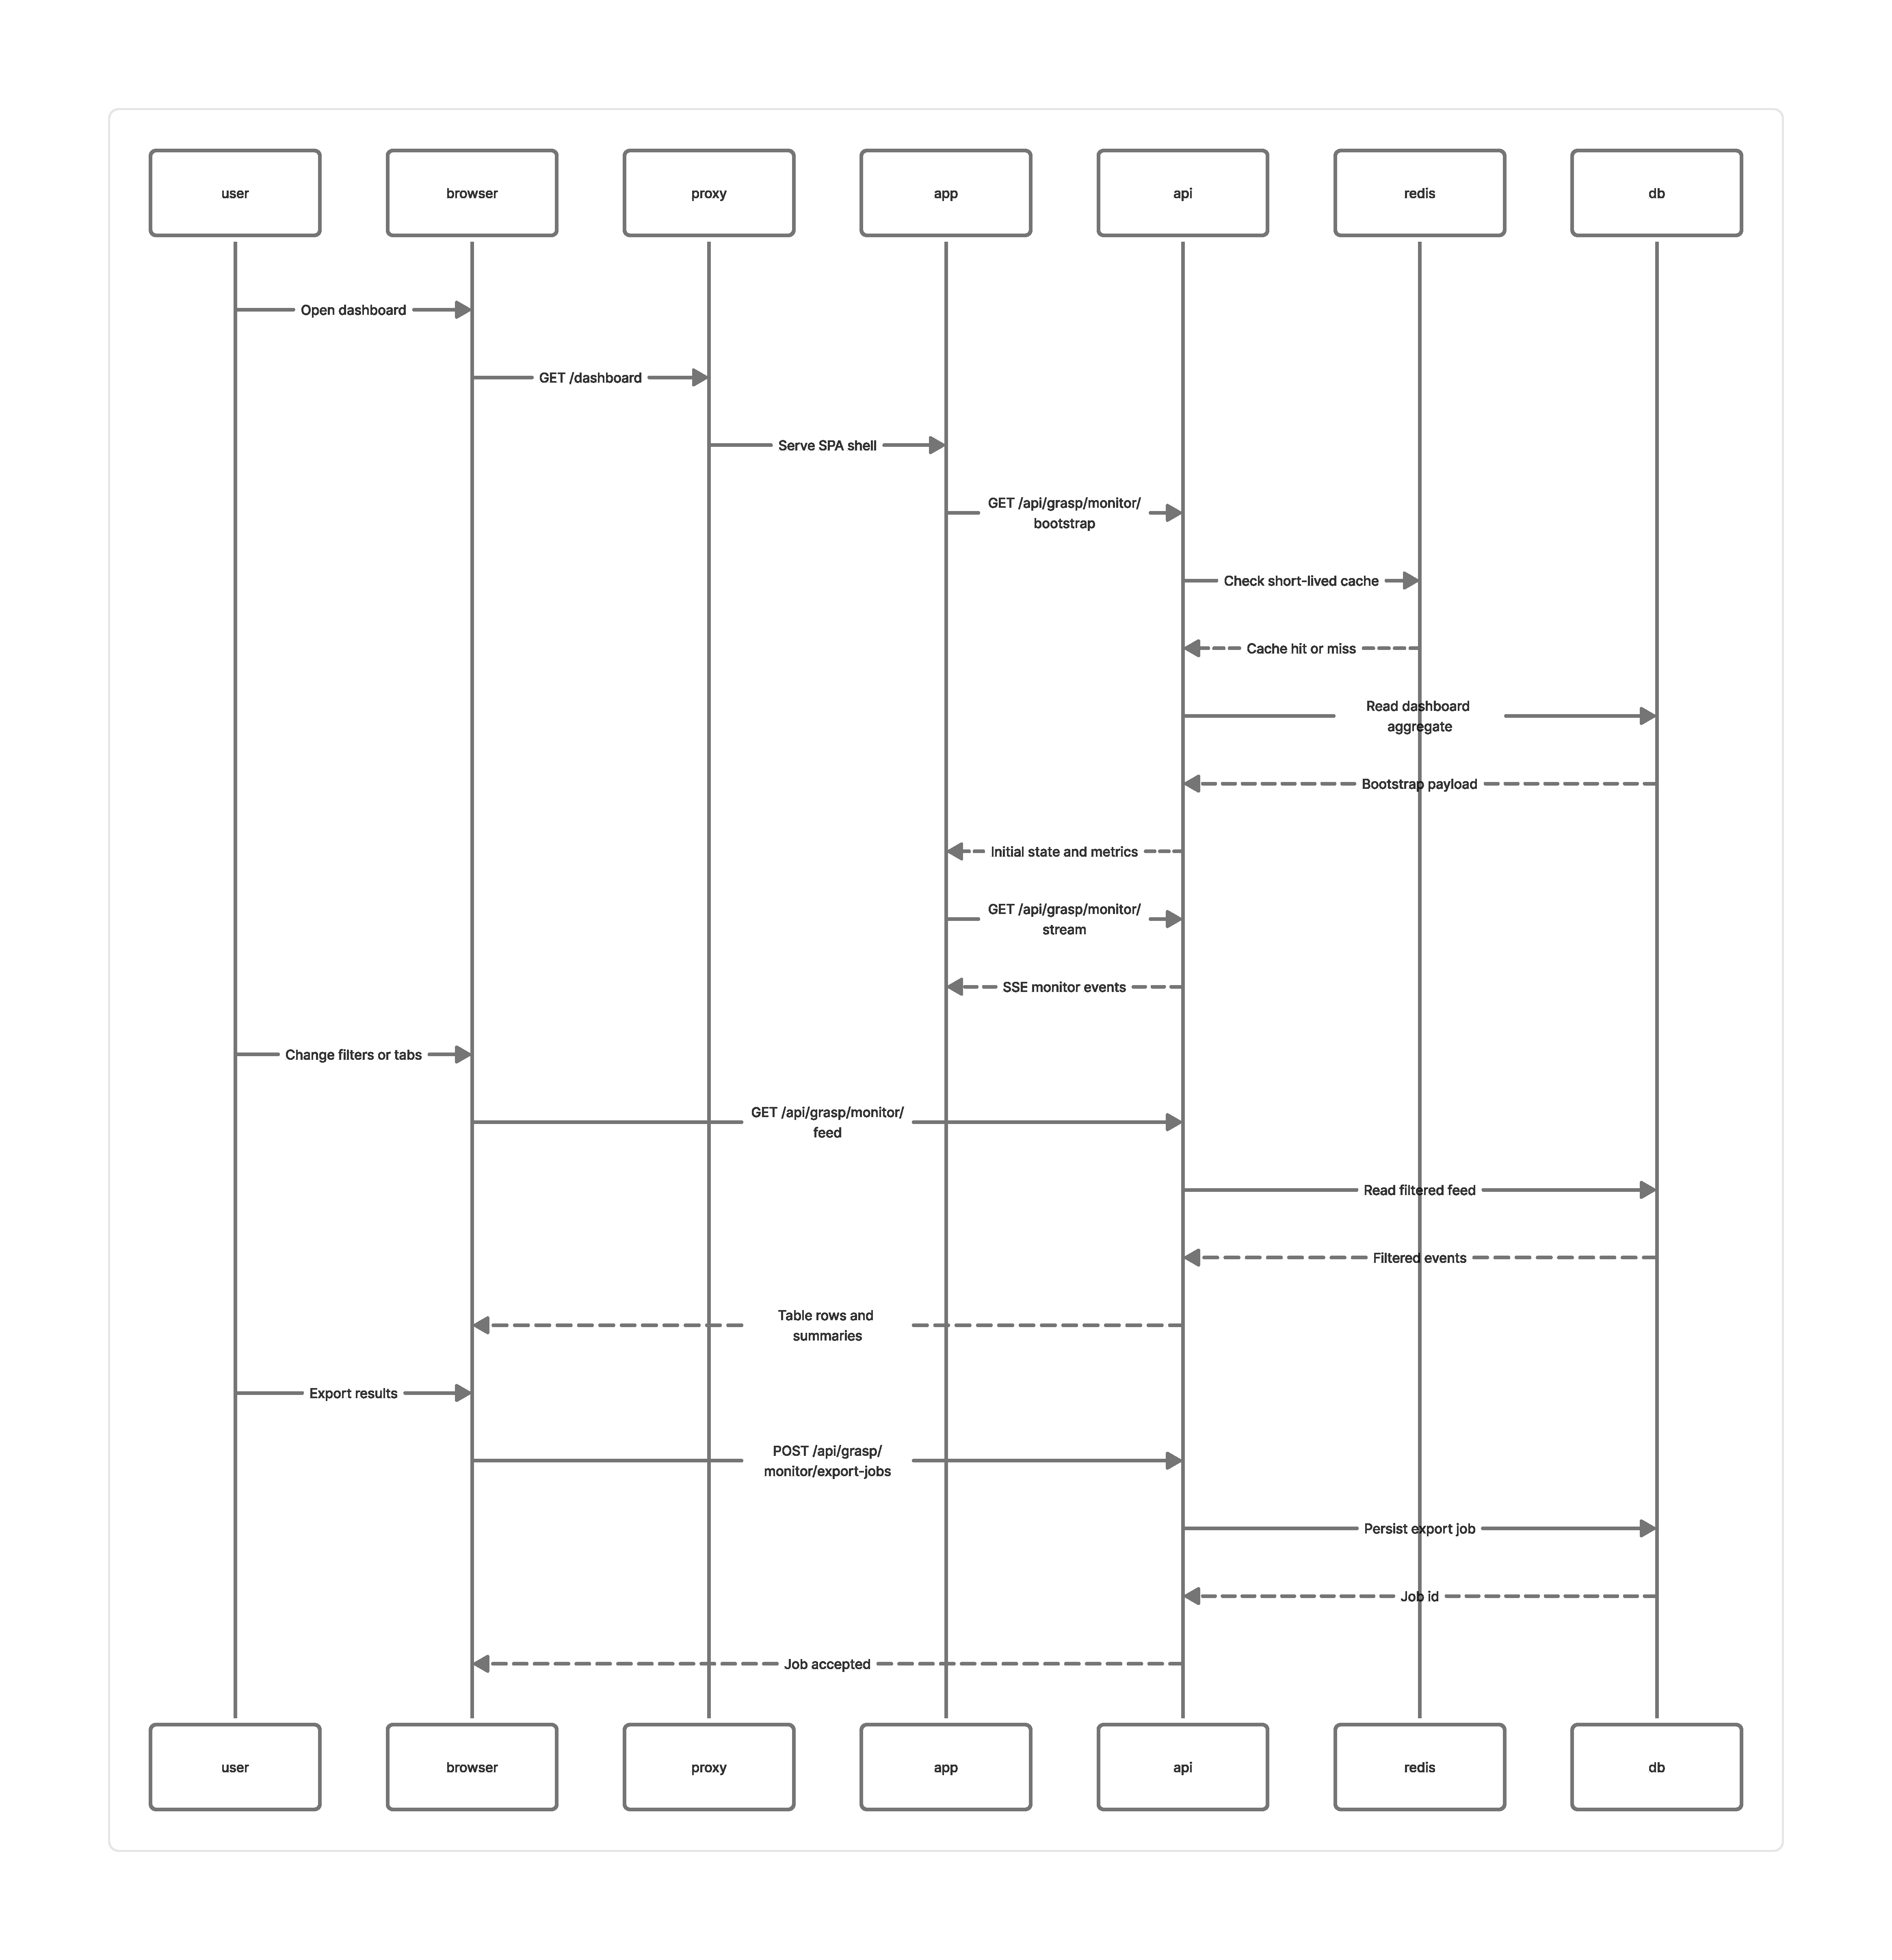
\includegraphics[width=\linewidth,height=.82\textheight,keepaspectratio]{fig/gfshield/gfshield-front-flow.pdf}
  \caption{Functional flow of the web client and its \ac{api} queries.}
  \label{fig:front-flow}
\end{figure}

\begin{landscape}
\begin{figure}[p]
  \centering
  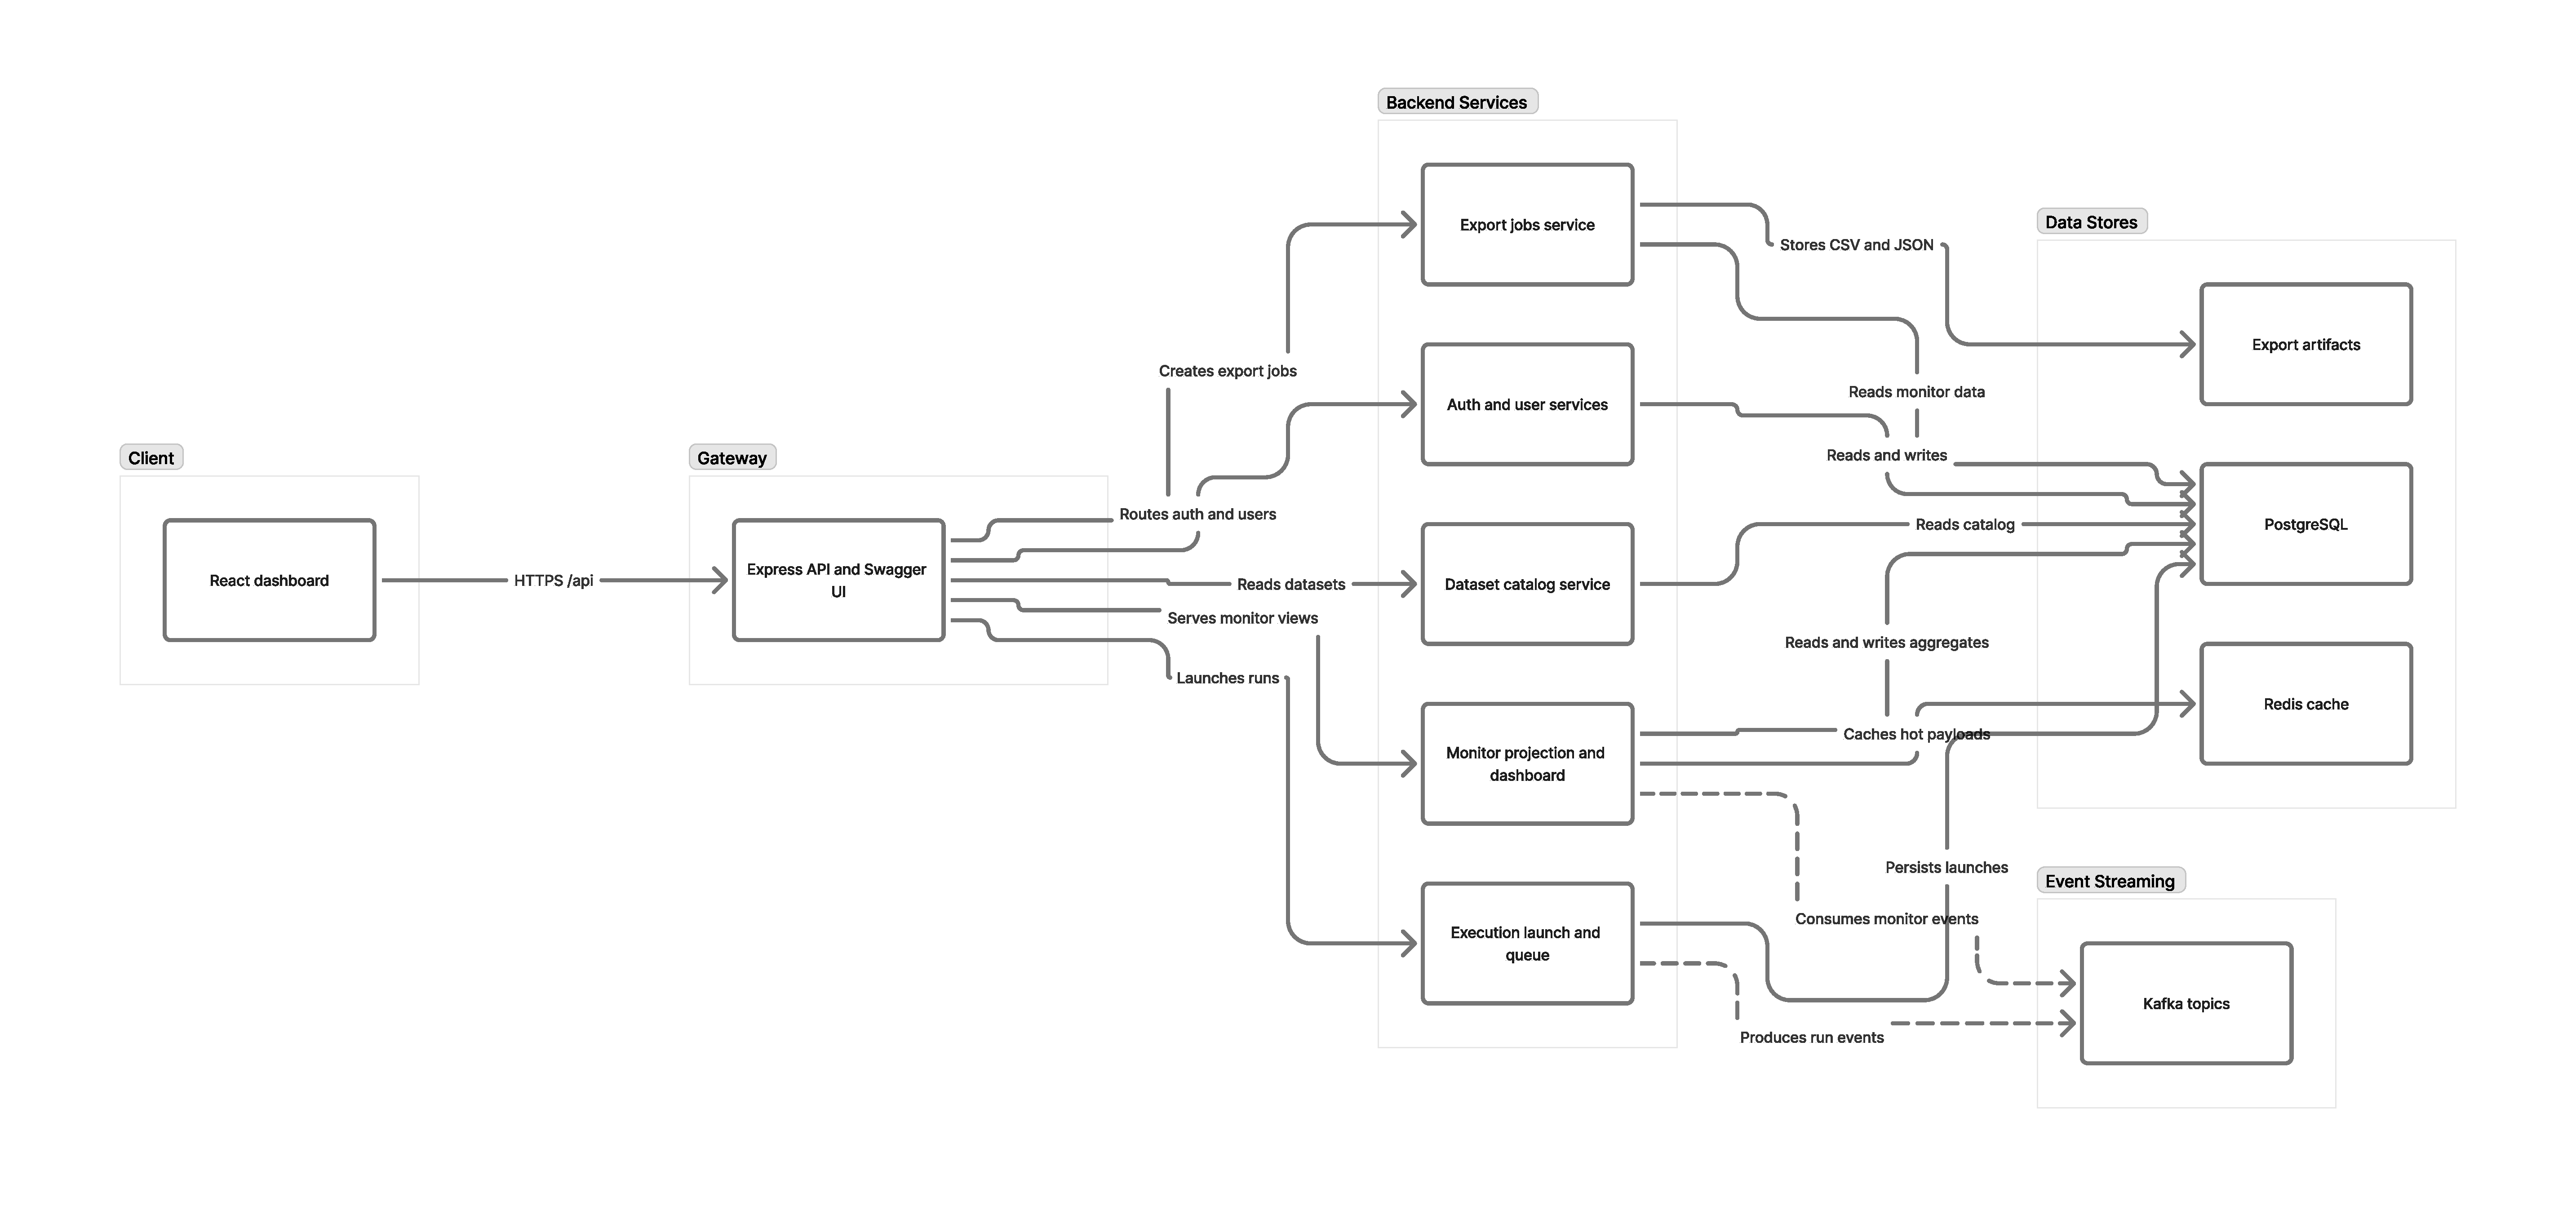
\includegraphics[width=.96\linewidth,height=.82\textheight,keepaspectratio]{fig/gfshield/gfshield-backend-architecture.pdf}
  \caption{Backend services, data stores, and messaging integration.}
  \label{fig:backend-architecture}
\end{figure}
\end{landscape}

Figures~\ref{fig:execution-lifecycle} through~\ref{fig:backend-architecture} complement the abstract view with the implemented flows. Interface captures, \ac{api} documentation, and supporting diagrams are provided in Appendices~\ref{app:frontend},~\ref{app:video-docs}, and~\ref{app:diagrams}.

\section{Reference Configuration and Reproducibility}

Table~\ref{tab:container-resources} records the local configuration defined by three files:
\begin{itemize}
  \item \path{docker-compose.yml};
  \item \path{docker-compose.local.yml};
  \item \path{webservice/api/docker-compose.db.yml}.
\end{itemize}
Values are per-container limits. The server preset increases some of these limits and must therefore not be mixed into an experimental comparison without an explicit record.

\begin{table}[!htb]
  \centering
  \scriptsize
  \caption{Resources and concurrency of the local reference configuration.}
  \label{tab:container-resources}
  \begin{tabularx}{\linewidth}{@{}Xc c c X@{}}
    \toprule
    \textbf{Service group} & \textbf{Count} & \textbf{CPU/unit} & \textbf{RAM/unit} & \textbf{Concurrency/configuration} \\
    \midrule
    DRG: IG, GR, SU, and ReliefF & 4 & 1.50 & 1536 MB & asynchronous pool: core 2, maximum 4, queue 80 \\
    DLS: Bit Flip, IWSS, and IWSSR & 3 & 1.00 & 1536 MB & one Kafka consumer per service \\
    VND, RVND, and verifier & 3 & 0.75 & 768 MB & one Kafka consumer per service \\
    Kafka & 1 & 1.00 & 1024 MB & six partitions; replication 1 \\
    ZooKeeper & 1 & 0.50 & 256 MB & client port 2181 \\
    Kafbat UI & 1 & 0.50 & 512 MB & internal Kafka client \\
    PostgreSQL & 1 & 0.50 & 512 MB & local database configuration \\
    Redis & 1 & 0.25 & 256 MB & AOF persistence and snapshots configured \\
    \bottomrule
  \end{tabularx}
\end{table}

The host identified as the execution server was inspected on August 25, 2026. The machine, identified by the operating system as \texttt{mc2-server-01}, has two Intel Xeon E5-2620 v4 processors at 2.10 GHz, with eight cores and two threads per core in each socket, totaling 16 physical cores and 32 logical processors in two NUMA nodes. Docker detected 67,447,271,424 bytes of memory (64,322.73 MiB; approximately 62.8 GiB), and the system had 8 GiB of swap. The environment runs Ubuntu 18.04.6 LTS, x86-64, and Linux kernel 4.15.0-213-generic. The inspection found Docker Engine/client 24.0.2, API 1.43, the \texttt{overlay2} storage driver, the \texttt{cgroupfs} cgroup driver, \texttt{docker compose} 2.18.1, and the \texttt{docker-compose} executable 2.30.3.

Docker labels linked the running services to the \texttt{g-fshield} project and to the overlay of \path{docker-compose.yml} with \path{docker-compose.server.yml}. Table~\ref{tab:server-container-resources} records the effective limits observed. There was one instance of each service; neither Swarm mode nor additional container replication was active. PostgreSQL and Redis belonged to a second composition formed by \path{webservice/api/docker-compose.db.yml} and \path{webservice/api/docker-compose.db.server.yml}. The \ac{api} and web client did not appear in the container list, so no observed limit is attributed to them.

From the repository root, the commands corresponding to the files recorded in the labels are:
\begin{lstlisting}[basicstyle=\ttfamily\footnotesize,breaklines=true,columns=fullflexible]
docker compose -f docker-compose.yml -f docker-compose.server.yml up -d
docker compose -f webservice/api/docker-compose.db.yml -f webservice/api/docker-compose.db.server.yml up -d
\end{lstlisting}
These commands reconstruct the observed composition; they do not replace terminal history or a manifest confirming the options used in the campaign.

\begin{table}[!htb]
  \centering
  \scriptsize
  \caption{Effective limits on the inspected server.}
  \label{tab:server-container-resources}
  \begin{tabularx}{\linewidth}{@{}Xc c c X@{}}
    \toprule
    \textbf{Service group} & \textbf{Count} & \textbf{CPU/unit} & \textbf{RAM/unit} & \textbf{Concurrency/configuration} \\
    \midrule
    DRG: IG, GR, SU, and ReliefF & 4 & 2.00 & 2048 MB & pool: core 3, maximum 6, queue 150 \\
    DLS: Bit Flip, IWSS, and IWSSR & 3 & 1.50 & 2048 MB & one Kafka consumer per service \\
    VND, RVND, and verifier & 3 & 1.00 & 1024 MB & one Kafka consumer per service \\
    Kafka & 1 & 2.00 & 2048 MB & six partitions; replication 1 \\
    ZooKeeper & 1 & 0.75 & 512 MB & one instance \\
    Kafbat UI & 1 & 1.00 & 2048 MB & one instance \\
    PostgreSQL & 1 & 1.00 & 1024 MB & one instance \\
    Redis & 1 & 0.25 & 256 MB & one instance \\
    \bottomrule
  \end{tabularx}
\end{table}

Directory \path{/home/idscps/nicolas/graspy2} supplied the implementation of Monolith~1. Directory \path{/home/idscps/nicolas/Graspy} supplied that of Monolith~2. For the formal campaign, both were rebuilt as versioned images and run as one container per arm under the same aggregate ceiling. Monolith~1 ranks features with Gain Ratio, constructs a five-feature subset from cutoff 30, and applies Bit-Flip for at most 100 local iterations. Monolith~2 uses Gain Ratio, constructs five features from an RCL of size 30, and applies IWSS under VND for at most 100 iterations. Both receive the same immutable training, validation, and test splits, seeds 42--49, 3,000-s limit, maximum of 500 accepted improvements, and minimum improvement 0.0001.

During formal search, both monoliths use the same Weka J48 evaluator and validation macro-F1. The best validation solution is then evaluated once on test. This adaptation removes historical classifier and metric-scale differences while preserving the GR--BF and GR--IWSS comparator algorithms. It does not make the monoliths algorithmically identical to G-FShield, whose legacy internal objective remains different.

The four DRG services expose ports 8086--8089; Bit Flip, IWSS, IWSSR, and the verifier use 8082--8085; RVND and VND use 8090 and 8091. Kafka exposes 19092, ZooKeeper 2181, JMX 9999, and Kafbat UI 8080. The \ac{api}, web client, PostgreSQL, and Redis use 4000, 3000, 5432, and 6379 by default. Datasets and CSVs are bind volumes for the \texttt{datasets/} and \texttt{metrics/} directories; PostgreSQL and Redis use named volumes.

The Java images are built with Maven 3.9.4 and Eclipse Temurin 17 and run on the Temurin 17 JRE. Most evaluation modules declare Weka 3.8.0; the SU service \texttt{pom.xml} contains duplicate declarations for 3.8.6 and 3.8.0, so the resolved dependency tree must be archived. DRG modules use Spring Boot 3.0.0, and DLS modules use Spring Boot 2.7.5. The infrastructure pins these images:
\begin{itemize}
  \item \path{confluentinc/cp-kafka:7.4.0};
  \item \path{confluentinc/cp-zookeeper:7.4.0};
  \item \path{ghcr.io/kafbat/kafka-ui:v1.4.2};
  \item \path{postgres:14};
  \item \path{redis:7-alpine}.
\end{itemize}
The optional mode that runs the web layer in containers uses \texttt{node:24}; the project declares Express 4.21.1, React 18.2.0, and Vite 8.0.3. The Compose files do not impose CPU and RAM limits on the \ac{api} and web client started by the scripts; these limits must also be fixed for a performance reproduction.

\subsection{Formal campaign manifest}

The formal campaign identifier is \texttt{gfshield-10d-2026-v1}. Its tag is \texttt{experiment-10d-v1}, and the launch commit is \texttt{66565b865a7b}. Images were built from commit \texttt{b38eff3ed9c1}; the manifest preserves the SHA-256 ID of each local image and the digests of Kafka 7.4.0 and ZooKeeper 7.4.0. The manifest, resolved Compose file, and host provenance have their own hashes. Each run also archives its command, resolved Compose file, logs, metrics, telemetry, final result, and a checksum manifest.

The file \path{experiments/10-day-campaign/frozen-compose.yaml} freezes the services used by the protocol. Each distributed configuration starts one RCL generator, VND or RVND, all three BF/IWSS/IWSSR operators, the verifier, Kafka, and ZooKeeper. There is one consumer per service and one logical execution partition; Kafka uses six partitions, replication factor one, and automatic topic creation. Java services use Temurin 17; the common evaluator uses Weka 3.8.6. The monoliths are separate images derived from \path{graspy2} and \path{Graspy}. Every arm uses \texttt{--cpuset-cpus 8-15}, \texttt{--cpuset-mems 1}, and an aggregate ceiling of eight CPUs and 16~GiB. The host kernel does not expose Docker swap accounting; the memory limit was enforced, but a separate swap limit could not be verified.

Data are mounted read-only at \path{/data} or \path{/datasets}; results, logs, and metrics use bind volumes specific to each \texttt{run\_id}. Generator ports are published only on \texttt{127.0.0.1} during execution; Kafka and the remaining services communicate over the composition's internal network. The web layer is not part of the campaign's measured path.

The durable server launch was:

\begin{lstlisting}[basicstyle=\ttfamily\footnotesize,breaklines=true,columns=fullflexible]
python3 experiments/10-day-campaign/campaign_supervisor.py \
  --manifest experiments/10-day-campaign/manifest.yaml \
  --state experiments/10-day-campaign/state/campaign-state.json \
  --supervisor-state experiments/10-day-campaign/state/supervisor-state.json \
  --log experiments/10-day-campaign/logs/campaign-supervisor.log \
  --output-root experiments/10-day-campaign/results
\end{lstlisting}

The supervisor preserves the absolute deadline, checks free storage, terminates process groups, and limits restarts. It did not restart in the reported execution. The campaign produced 216 valid results for 27 arms and eight seeds, plus 12 preserved invalid attempts that were retried. The repository contains \path{experiments/10-day-campaign/analyze_results.py}, which verifies checksums, normalizes metrics, and recreates tables and figures. Reproduction still requires access to the images or rebuilding them at the recorded commit, the corpus matching the recorded hashes, and a compatible host; dynamic CPU frequency, external containers, and physical-hardware limitations are not eliminated by containerization.

\section{Synthesis}

\textit{G-FShield} integrates independent GRASP-FS construction branches, local-search controllers and operators, messaging, and verification of observed best results. A web layer queries data held in persistent storage. The input contract, pseudocode, manifest, and container configuration delimit implementation and campaign. The architecture provides decoupling, inspection, and evolution; the campaign establishes experimental traceability, while scalability, fault tolerance, and portability across hosts remain properties to evaluate.
